\documentclass{standalone}

\usepackage{circuitikz}

\begin{document}

% INT_AY20_MP3_L27_Fig03_Rect_loop_through_field.png

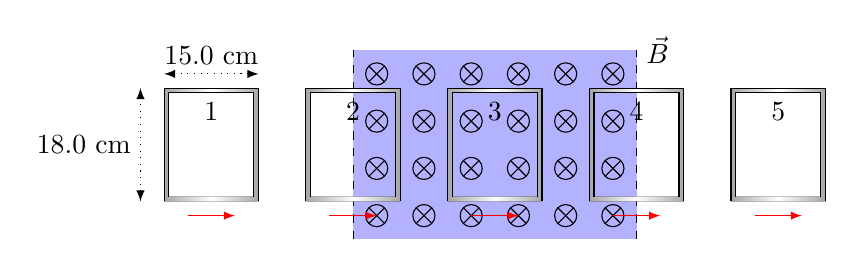
\begin{tikzpicture}[> = latex]

	% Definition
	
	\def\L{0.6}		% Length scale for magnetic field

	% Magnetic field
	
	\filldraw [draw = none, fill = blue!30] (-3 * \L, -2 * \L) rectangle (3 * \L, 2 * \L);
	
	\foreach \x in {-2.5, -1.5, -0.5, 0.5, 1.5, 2.5}
	\foreach \y in {-1.5, -0.5, 0.5, 1.5}
	{
		\draw (\x * \L, \y * \L) circle (4 pt);
		\draw (\x * \L, \y * \L) ++ (45 : 4 pt) -- ++ (225 : 8 pt);
		\draw (\x * \L, \y * \L) ++ (135 : 4 pt) -- ++ (315 : 8 pt);
	}
	
	\begin{scope}[dashed]
	
		\draw (-3 * \L, -2 * \L) -- (-3 * \L, 2 * \L);
		\draw (3 * \L, -2 * \L) -- (3 * \L, 2 * \L) node [right] {${\vec B}$};
	
	\end{scope}
	
	% Rectangle to left of field
	
	\filldraw [even odd rule, left color = gray!70, right color = gray!70, middle color = white, draw = black]
		(-7 * \L, -1.2 * \L) -- (-7 * \L, 1.2 * \L) -- (-5 * \L, 1.2 * \L) -- (-5 * \L, -1.2 * \L)
		(-6.9 * \L, -1.1 * \L) -- (-6.9 * \L, 1.1 * \L) -- node [midway, below] {1} (-5.1 * \L, 1.1 * \L) -- (-5.1 * \L, -1.1 * \L);
		
	% Loop dimension indicators
	
	\begin{scope}[<->, dotted]
	
		\draw (-7 * \L, 1.5 * \L) -- node [midway, above] {15.0 cm} (-5 * \L, 1.5 * \L);
		\draw (-7.5 * \L, -1.2 * \L) -- node [midway, left] {18.0 cm} (-7.5 * \L, 1.2 * \L);
	
	\end{scope}
		
	% Rectangle entering field
	
	\filldraw [even odd rule, left color = gray!70, right color = gray!70, middle color = white, draw = black]
		(-4 * \L, -1.2 * \L) -- (-4 * \L, 1.2 * \L) -- (-2 * \L, 1.2 * \L) -- (-2 * \L, -1.2 * \L)
		(-3.9 * \L, -1.1 * \L) -- (-3.9 * \L, 1.1 * \L) -- node [midway, below] {2} (-2.1 * \L, 1.1 * \L) -- (-2.1 * \L, -1.1 * \L);
	
	% Rectangle inside field
	
	\filldraw [even odd rule, left color = gray!70, right color = gray!70, middle color = white, draw = black]
		(-\L, -1.2 * \L) -- (-\L, 1.2 * \L) -- (\L, 1.2 * \L) -- (\L, -1.2 * \L)
		(-0.9 * \L, -1.1 * \L) -- (-0.9 * \L, 1.1 * \L) -- node [midway, below] {3} (0.9 * \L, 1.1 * \L) -- (0.9 * \L, -1.1 * \L);
		
	% Rectangle leaving field
	
	\filldraw [even odd rule, left color = gray!70, right color = gray!70, middle color = white, draw = black]
		(4 * \L, -1.2 * \L) -- (4 * \L, 1.2 * \L) -- (2 * \L, 1.2 * \L) -- (2 * \L, -1.2 * \L)
		(3.9 * \L, -1.1 * \L) -- (3.9 * \L, 1.1 * \L) -- node [midway, below] {4} (2.1 * \L, 1.1 * \L) -- (2.1 * \L, -1.1 * \L);
	
	% Rectangle to right of field
	
	\filldraw [even odd rule, left color = gray!70, right color = gray!70, middle color = white, draw = black]
		(7 * \L, -1.2 * \L) -- (7 * \L, 1.2 * \L) -- (5 * \L, 1.2 * \L) -- (5 * \L, -1.2 * \L)
		(6.9 * \L, -1.1 * \L) -- (6.9 * \L, 1.1 * \L) -- node [midway, below] {5} (5.1 * \L, 1.1 * \L) -- (5.1 * \L, -1.1 * \L);
		
	% Velocity vectors
	
	\begin{scope}[->, red]
	
		\draw (-6.5 * \L, -1.5 * \L) -- (-5.5 * \L, -1.5 * \L);
		\draw (-3.5 * \L, -1.5 * \L) -- (-2.5 * \L, -1.5 * \L);
		\draw (-0.5 * \L, -1.5 * \L) -- (0.5 * \L, -1.5 * \L);
		\draw (2.5 * \L, -1.5 * \L) -- (3.5 * \L, -1.5 * \L);
		\draw (5.5 * \L, -1.5 * \L) -- (6.5 * \L, -1.5 * \L);
	
	\end{scope}
	
\end{tikzpicture}

\end{document}